\documentclass[12pt,letterpaper,noanswers]{exam}
%\usepackage{color}
\usepackage[usenames,dvipsnames,svgnames,table]{xcolor}
\usepackage[margin=0.9in]{geometry}
\renewcommand{\familydefault}{\sfdefault}
\usepackage{multicol}
\pagestyle{head}
\definecolor{c02}{HTML}{FFBBBB}
\definecolor{c03}{HTML}{FFDDDD}
\header{AM 108 Problem Set 06}{}{{\colorbox{c02}{\makebox[3.0cm][l]{Due Fri Mar 10}}}\\ at noon p.\thepage}
\runningheadrule
\headrule
\usepackage{diagbox}
\usepackage{graphicx} % more modern
%\usepackage{subfigure} 
\usepackage{amsmath} 
\usepackage{amssymb} 
%\usepackage{gensymb} 
%\usepackage{natbib}
\usepackage{hyperref}
%\usepackage{enumitem}
%\setlength{\parindent}{0pt}
%\usepackage{setspace}
%\pagestyle{empty}  
%\newcommand{\Sc}[0]{
%{\color{BlueViolet}\S}
%}
\usepackage{tcolorbox}
\usepackage[framed,numbered,autolinebreaks,useliterate]{mcode}

% \renewcommand{\labelenumii}{\theenumii}
% \renewcommand{\theenumii}{\theenumi-\arabic{enumii}.}

\newif\ifprintselans
\printselanstrue
%\printselansfalse
\newenvironment{selans}
{\ifprintselans
   \printanswers
   \renewcommand{\solutiontitle}{\noindent\textbf{Answer:}\par\noindent}
 \fi
}
{}

\newif\ifprintselsol
%\printselsoltrue
\printselsolfalse
\newenvironment{selsol}
{\ifprintselsol
   \printanswers
   \renewcommand{\solutiontitle}{\noindent\textbf{Solution:}\par\noindent}
 \fi
}
{}


\begin{document}
 \pdfpageheight 11in 
  \pdfpagewidth 8.5in

\noindent\textbf{Problem Set Instructions:}  
\begin{itemize}
\itemsep0pt
\item In your first attempt of the problem set problems, you are encouraged to treat the problem set as an open-notes quiz.  Work on it without consulting classmates, Ed, course staff, other people, other internet resources, or any solutions or answers.  Work on each problem, completing as much as you are able to, and making a note in your work whenever you become stuck or confused.
\item After your initial individual attempt, collaboration is encouraged (see guidelines below) as you continue to work on the problems.  You'll submit a pdf of this work as part of your problem set submission on Gradescope (and will also submit it on Canvas).
\item Submit the pdf of your problem set work with the problems written up in order (computational work should be included: it can be at the end of the pdf) on Canvas and access the solutions.
\item Complete the reflection questions below, and submit that reflection work, along with your problem set pdf, on Gradescope.
\end{itemize}
  
\noindent\textbf{Submission Instructions:}  
\begin{itemize}
\item Following the instructions above, upload a pdf of your work to Canvas.  Upload your reflection answers and the pdf to Gradescope.
\item If you would like to use mathematical software other than Mathematica, that's fine. 
\end{itemize}

\noindent\textbf{Late Work Policy:}
\begin{itemize}
\itemsep0pt
\item Problem sets are accepted up to eight hours late with no penalty (8pm Friday). 
\item Three 36 hour late days are available to every student (three extensions to 8pm on Saturday).  These late days are expected to be used for unexpected illness or other conflicts.
\item Additional late days are not typically 
available.
\item Problem sets are not accepted beyond the late deadline.
\end{itemize}

\noindent\textbf{Collaborating on Problem Sets:}  

\noindent Collaborating with classmates in planning and designing solutions to homework problems is encouraged.  Collaboration, cooperation, and consultation can all be productive.  Work with others to: 
\begin{multicols}{2}
\begin{itemize}
\itemsep-0.2em
    \item discuss the problem
    \item brainstorm
    \item walk through possible strategies
    \item outline solution methods
\end{itemize}   
\end{multicols}

\noindent For homework, you may consult or use:
\begin{multicols}{2}
\begin{itemize}
\itemsep-0.2em
    \item Course text (including answers in back)
    \item Your notes (taken during class)
    \item Class notes of other students
    \item Course handouts
    \item Canvas posts/Ed posts
    \item Computational tools such as Python, Mathematica, or Desmos
    \item Calculators
    \item Other books
    \item the Internet
\end{itemize}
\end{multicols}

\noindent You may:
\begin{itemize}
    \item Look at communal work while writing up your own solution
\end{itemize}

\noindent You may \textbf{not}:
\begin{itemize}
\itemsep-0.2em
    \item Look at the individual work of others while writing up your own solutions
    \item Post about problems online
\end{itemize}


\noindent Do \textbf{not} consult the following resources until after you think you have solved a problem, have fully written up your answer, and have submitted a pdf of your work to Canvas.
%\begin{multicols}{2}
\begin{itemize}
\itemsep-0.2em
    \item The text solution manual
    \item The posted solutions
    \item Other solutions (from previous years, from sites like Chegg or Math Stackexchange, etc)
\end{itemize}
%\end{multicols}


%\eject


% \begin{enumerate}
% \item Reflection questions

\section*{Reflection questions}
Submit these on Gradescope.
\begin{enumerate}
\item \begin{enumerate}
    \itemsep0pt
    \item When you worked on the problems individually, how did each problem go?
    \item Where did you get stuck or confused?  For any subpart where you were stuck or confused be specific.  \emph{For example 'I tried to use the hint for 3b, but I couldn't find a way to relate $r$ and $x$'.}
    \item What additional progress were you able to make when you consulted other people or additional resources?
    \item For each part of each problem, how did your work compare with the posted solution?  Identify similarities and differences.
\end{enumerate}  
\item For any problems you were not able to complete, what made them difficult to complete?  What did you learn from the posted solution?
\item What aspects of the course challenged you this week?  What did you do to address those challenges?  What topics/ideas/procedures do you not yet understand?
\item What did you understand the best this week?  What, if anything, do you understand better this week than you did in the past?
\item List the people that you worked with or consulted on the problem set problems.  This might include other students in the course, course instructors, or people who have previously taken the course.
\item Below, indicate how much of your time for this class has been doing the following activities:
	\begin{enumerate}
	\item Working on problem set problems or other practice problems alone
	\item Viewing preclass materials or reviewing course materials, including problem set solutions, alone
	\item Working on problem sets, reviewing notes, or discussing course topics with your classmates
	\item Working through supplementary materials
	\item Going to office hours
	\item Other (please specify)
	\end{enumerate}

\end{enumerate}


\section*{Problems}
\begin{questions}
\question (working with polar, 7.1.5, 7.3.3) 
\begin{parts}
\part (based on 7.1.5) 
 Show that the system $\dot{r} = r(1-r^2), \dot{\theta} = 1$ is equivalent to 
\begin{align*}
\dot{x} &= x - y - x(x^2+y^2) \\
\dot{y} &= x + y - y(x^2+y^2)
\end{align*}
where $x = r\cos\theta$ and $y = r\sin\theta$.

\emph{Recall the multivariable chain rule: $\dfrac{dx}{dt} = \dfrac{dr}{dt}\cos\theta - r\dfrac{d\theta}{dt}\sin\theta$.}



\emph{You are welcome to use Mathematica/Python for this; in that case explain how you used Mathematica/Python as part of your writeup (and submit the work as part of your pdf).}

\begin{solution}

\begin{align*}
x &= r \cos\theta \\
\dot x &= \dot r \cos\theta - r\sin\theta\dot\theta \\
&= r(1-r^2)\cos\theta - r\sin\theta \\
& = x(1-r^2) - y \\
&= x - y - x(x^2+y^2)
\end{align*}

\begin{align*}
y &= r \sin\theta \\
\dot y &= \dot r \sin\theta + r\cos\theta\dot\theta \\
&= r(1-r^2)\sin\theta + r\cos\theta \\
& = y(1-r^2) + x \\
&= x + y - y(x^2+y^2)
\end{align*}

See Mathematica work at end of file as well.
\end{solution}

\part Make a streamplot for the system above.  In addition, use numerical integration to create two trajectories: one that starts at $(0.01, 0)$ and one that starts at $(2,0)$.  Add those trajectories to your streamplot.

\emph{See sample Python/Mathematica files on Canvas}.
  %No need to analyze the system.

\begin{solution}

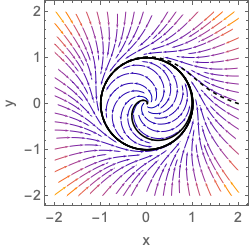
\includegraphics{img/PS07-1a.png}

See Mathematica at end of file.
\end{solution}




\part (7.3.3) Do this problem as written.
% Consider the system $\dot{x} = x - y - x^3, \dot{y} = x + y - y^3$.  Rewrite the system in polar coordinates, where $r^2 = x^2 + y^2, \tan\theta = \frac{y}{x}$.  Then construct a trapping region and use the Poincar\'e-Bendixson Theorem to show that the system has a closed trajectory.

% \emph{From the chain rule: $r\dot{r} = x\dot{x} + y\dot{y}$ and $\dot{\theta} = (x\dot{y} - y\dot{x})/r^2$.}

\emph{As above, you are welcome to use Mathematica/Python to help you; in that case explain how you used it as part of your writeup, include the code in the pdf, etc.}

\emph{Trapping regions for the Poincar\'e-Bendixson theorem need to be closed sets, so they need to include their boundary points.}

\begin{solution}

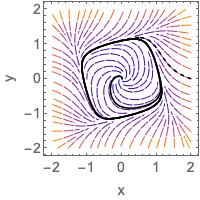
\includegraphics{img/PS06-1c.png}
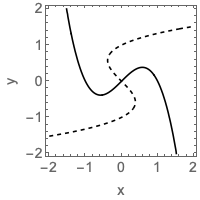
\includegraphics{img/PS06-1c2.png}

From this streamplot, the square bounded by $x = 2, y = 2, x = -2, y = -2$ traps all trajectories.  Check that:

$x = 2$:

$\dot x = 2-8-y = -6-y$ so for $-2\leq y \leq 2$ this is negative (and trajectories enter the square.

$x = -2$:

$\dot x = -2+8-y = 6-y$.  Positive for $-2\leq y \leq 2$ so trajectories point inwards on this line as well.

$y = 2$:

$\dot y = 2 - 8 + x = -6 + x$.  Negative/inward for $-2\leq x \leq 2$.

$y = -2$:

$\dot y = -2 + 8 + x = 6 + x$.  Positive/inward for $-2\leq x \leq 2$.

The square does trap all trajectories.  It has a fixed point within it, though, at $(0,0)$, so we can't use the Poincare-Bendixson theorem yet.

Trying to exclude a small square, I find the argument above does not work. 

I can see from the streamplot that trajectories spiral outwards, so look for a circle on which $\dot r > 0$.

\begin{align*}
r^2 &= x^2 + y^2 \\
r\dot r &= x\dot x + y\dot y \\
r\dot r &= x(x-y-x^3) + y(x+y-y^3) \\
r\dot r &= x^2 - xy - x^4 +xy + y^2 - y^4 \\
r\dot r &= r^2 - r^4(\cos^4 \theta + \sin^4\theta) \\
\dot r &= r - r^3(\cos^4 \theta + \sin^4\theta) \\
\dot r &= r(1 - r^2(\cos^4 \theta + \sin^4\theta))
\end{align*}

$\dot r$ is positive when $1>r^2(\cos^4\theta + \sin^4\theta)$ and negative when $1<r^2(\cos^4\theta + \sin^4\theta)$.

We'll identify the range of $\cos^4\theta + \sin^4\theta$ to figure out where it is negative vs positive.

To find extremal values, find $\theta$ such that 

\begin{align*}
    \frac{d}{d\theta} (\cos^4\theta + \sin^4\theta) &= 0 \\
    -4\cos^3\theta\sin\theta+4\sin^3\theta\cos\theta &= 0 \\
    2\cos\theta\sin\theta(\sin^2\theta - \cos^2\theta) = 0 \\
    \sin 2\theta (-\cos 2\theta) &= 0 \\
\end{align*}
Zeros occur for $\theta = k\pi/4$ for $k$ and integer.

Either $\cos^4 \theta = 0$ and $\sin^4\theta = 1$ (or vice versa) so $\cos^4\theta + \sin^4\theta = 1$ or $\cos^4\theta = (\sqrt{2}/2)^4 = \sin^4\theta$ so $\cos^4\theta + \sin^4\theta = 1/2$.

$\dot r = r(1-k r^2)$ where  $\frac{1}{2}\leq k \leq 1$.  So $\dot r < 0$ on $r = 2$ (for all $\theta$) and $\dot r>0$ on $r = 1/4$ (for all $\theta$).

$1/4 \leq r \leq 2$ is a trapping region that contains no fixed points.  By the Poincare-Bendixson theorem, there is a closed orbit within that region.

\end{solution}


\end{parts}




% \question (7.2.9) Read about gradient systems in the text, and do this problem as written.  For (c) there may be a typo in your text.  The system should be $\dot x = -2xe^{x^2+y^2}$, $\dot y = -2y e^{x^2+y^2}$.


\question (inspired by 7.2.12) Consider the system
\begin{align*}
\dot{x} &= -x + 2y^3-2y^4 \\ 
\dot{y} &= -x-y+xy
\end{align*}
\begin{parts}
\part Find the nullclines of the system and sketch or plot them. 



\emph{It will be easier to find a function of the form $x=g(y)$ for the $x$ nullcline.}


\begin{solution}
The $x$ nullcline is implicitly $x=2y^3-2y^4$ and the $y$ nullclines is $y=-x/(1-x)$.  In the next part it will be beneficial to know that we can write the $y$ nullcline as $x=-y/(1-y)$. The $y$ nullcline has a horizontal asymptote of $y=1$ and a vertical asymptote of $x=1$.  The $x$ nullcline opens to the left (has a max at y=3/4). Sketching these curves yields:\\
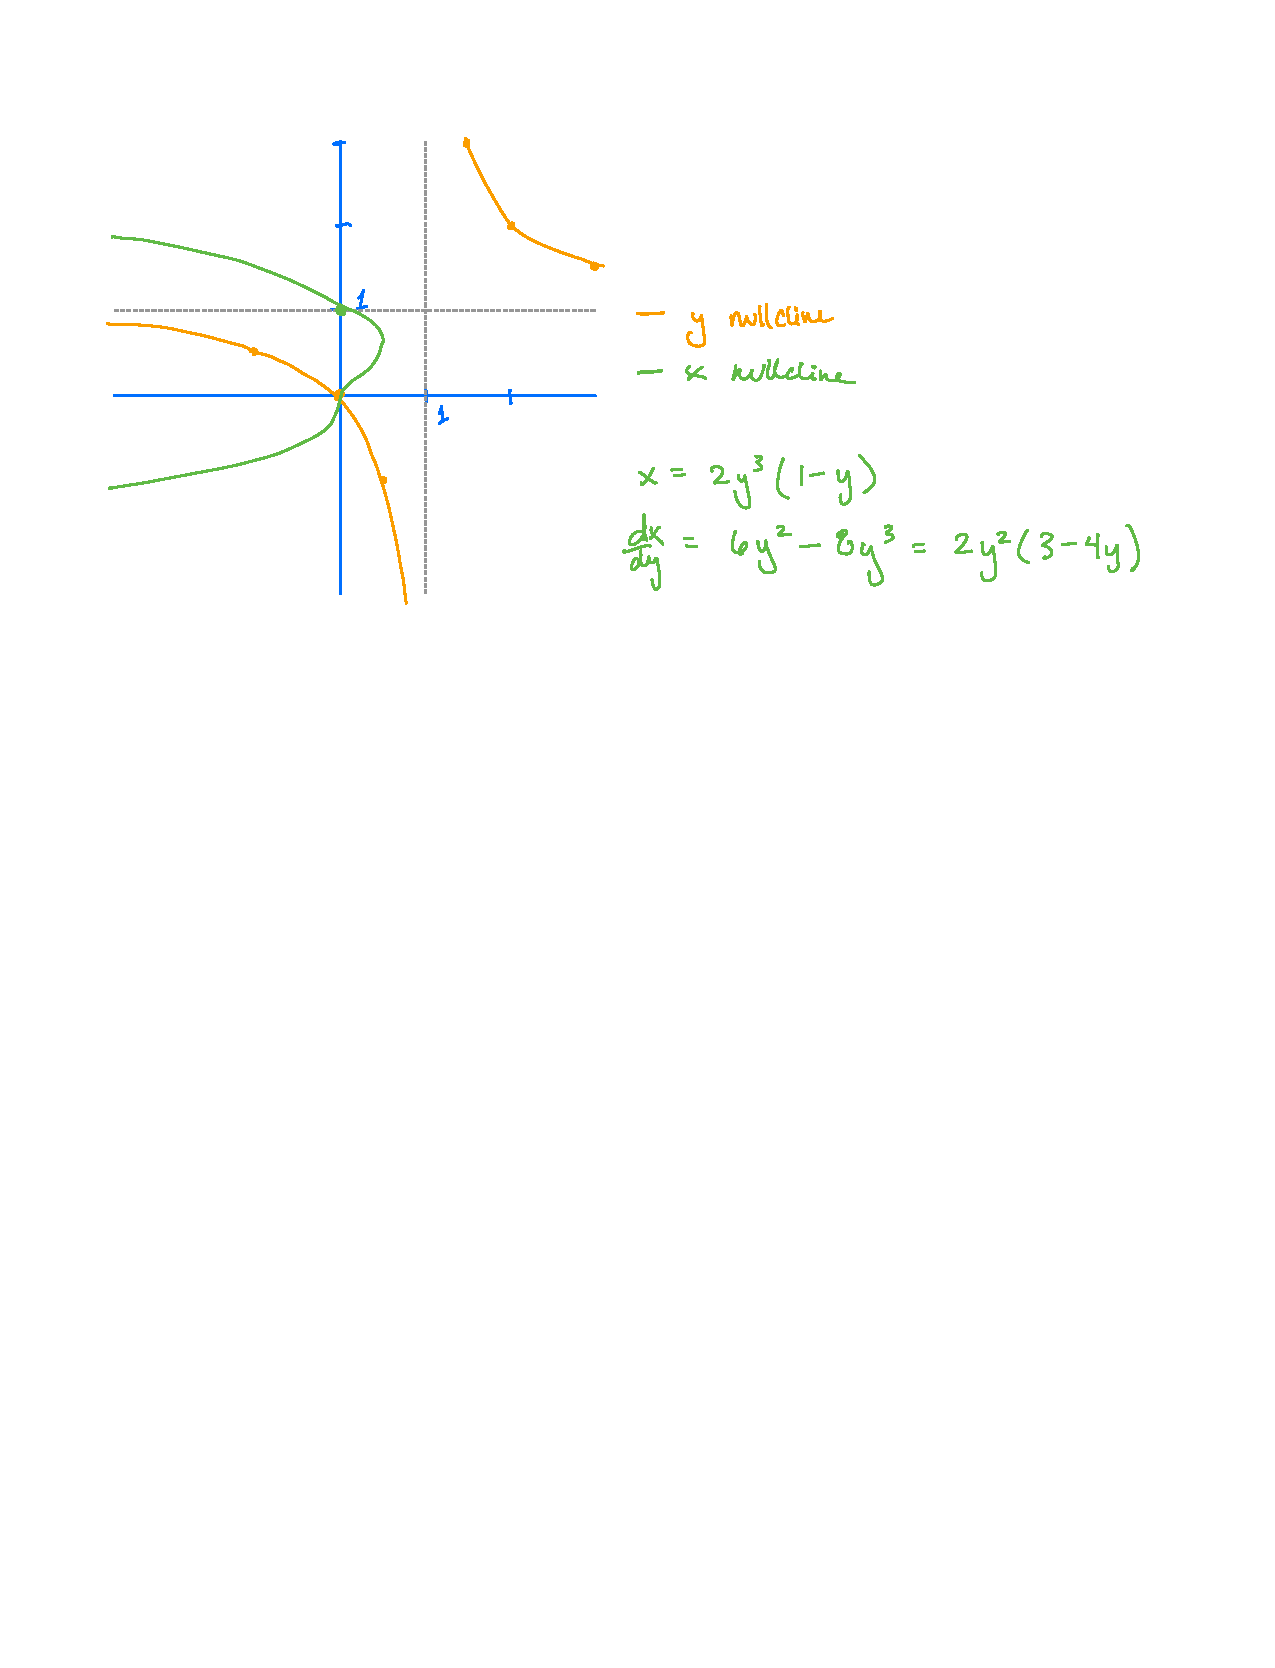
\includegraphics[width=6in]{img/H-07-2a}
\end{solution}

\part Argue why there can only be one equilibrium in this system and find it.

\begin{solution}
The $x$ nullcline is increasing for $y$ in  the interval $(-\infty,3/4)$ and decreasing in the interval $(3/4,\infty)$.  Since the $y$ nullcline is strictly decreasing for $y$ in the interval $(-\infty,1)$ so the curves can intersect at most once on the interval $(-\infty,3/4)$ and perhaps other times on the interval $[3/4,1)$.  From our sketch we can see that on $(-\infty,3/4)$ they intersect at (0,0).  On $[3/4,1)$, the $x$ nullcline is always greater than $y=1$ and the $y$ nullcline is always less than $y=1$, so they do not intersect.
\end{solution}


\part Compute the index of the fixed point.  Does this calculation allow you to rule out/rule in a limit cycle?

\begin{solution}
We will find the stability of the fixed point, if it is a hyperbolic fixed point, then we can use what we know about the index (saddles have index $-1$ and all other hyperbolic fixed points have index $1$) to determine the index of the point.\\

The Jacobian for the system is
\[J=\left[\begin{array}{cc}
-1 & 6y^2-8y^3\\
-1+y&-1+x\\
\end{array}\right]\]
so at $(0,0)$ we have
\[J=\left[\begin{array}{cc}
-1 & 0\\
-1&-1\\
\end{array}\right]\]
which has trace of $-2$ and determinant of $1$ so the fixed point is an attracting equilibrium and the index is 1.\\

Since limit cycles must surround equilibria where the sum of their indexes sum to 1, we cannot rule out a limit cycle with this method.
\end{solution}

\part Look in the text for the definition of a gradient system.  Determine whether the system is a gradient system. Does this determination allow you to rule out/rule in a limit cycle?

\begin{solution}
If we take the partial derivative with respect to $y$ of the $x$-component vector field and the partial derivative with respect to $x$ of the $y$-component vector field and the two computation are equal, then the system is a gradient system.\\

We have
\[\frac{\partial}{\partial y}(-x+2y^3-2y^4)=6y^2-8y^3\]
and
\[\frac{\partial}{\partial x}(-x-y+xy)=-1+x\]
which are not equal.  So the system isn't a gradient system and we can't rule out a limit cycle with this method.
\end{solution}


\item Assume you have a trajectory that is a closed orbit.  How does having a function, $V(x,y)$, that is decreasing on non-fixed point trajectories lead to a contradiction?

\emph{Motion on a closed trajectory is periodic, so $(x(t),y(t))$ is periodic on such a trajectory.}

\begin{solution}
Consider a trajectory that is a closed orbit with period $T$.  At time zero, the position is $(x_0,y_0)$ with $V$ at time zero given by $V(x_0, y_0)$.  At time $T$ the position is $(x_0,y_0)$ again, so $V(x(T),y(T)) = V(x_0,y_0)$, this $V$ must be periodic on a closed orbit.

$V$ cannot be periodic and also always decreasing, so there is a contradition.
\end{solution}

\part Determine whether the system has a Liapunov function of the form $V(x,y) =  x^m + a y^n$. (Look in the text for a definition).  Does this determination allow you to rule out/rule in a limit cycle?

\emph{You are welcome to use Python/Mathematica for this; be sure to describe your setup in your writeup and to submit your code on Canvas.}

\begin{solution}
\begin{align*}
\frac{dV}{dt} &= mx^{m-1}\dot x + nay^{n-1}\dot y \\
&= mx^{m-1}(-x+2y^3 - 2y^4) + nay^{n-1}(-x-y+xy) \\
&= -mx^m + 2mx^{m-1}y^3 - 2mx^{m-1}y^4 - nay^{n-1}x-nay^n+nay^n x \\
\end{align*}  

We need to eliminate all terms with odd exponents.  $x^{m-1}y^3$, $x^{m-1}y^4$, $y^{n-1}x, y^n x$.  Set $n = 4$ and $m=2$.

\begin{align*}
\frac{dV}{dt} &= 2x\dot x + 4ay^{3}\dot y \\
&= -2x^2 + 4xy^3 - 4xy^4 - 4ay^3x-4ay^4+4ay^4 x \\
&= -2x^2 + xy^3(4-4a) +xy^4(-4 +4a)-4ay^4 \\
\end{align*}  

Set $a = 1$.  $\frac{dV}{dt} = -2x^2 - 4y^4 \leq 0$.  This is decreasing everywhere but $(0,0)$, so there are no closed trajectories.

\end{solution}

\end{parts}

\question (inspired by 4.5.3) Read the intro/background to question 4.5.3 in the text.
\begin{parts}
\part Identify the threshold and the rest state in the system by sketching the vector field on the line segment $[0,2\pi]$ and also on the circle. Describe the behavior of the system and sketch two solutions for if the initial condition is on either side of the threshold.

\begin{solution}
When $\mu$ is slightly less than 1, is is very close to the amplitude of the sine wave, so there will only be a small portion of the vector field that is negative. We can sketch that with our knowledge of sine:\\
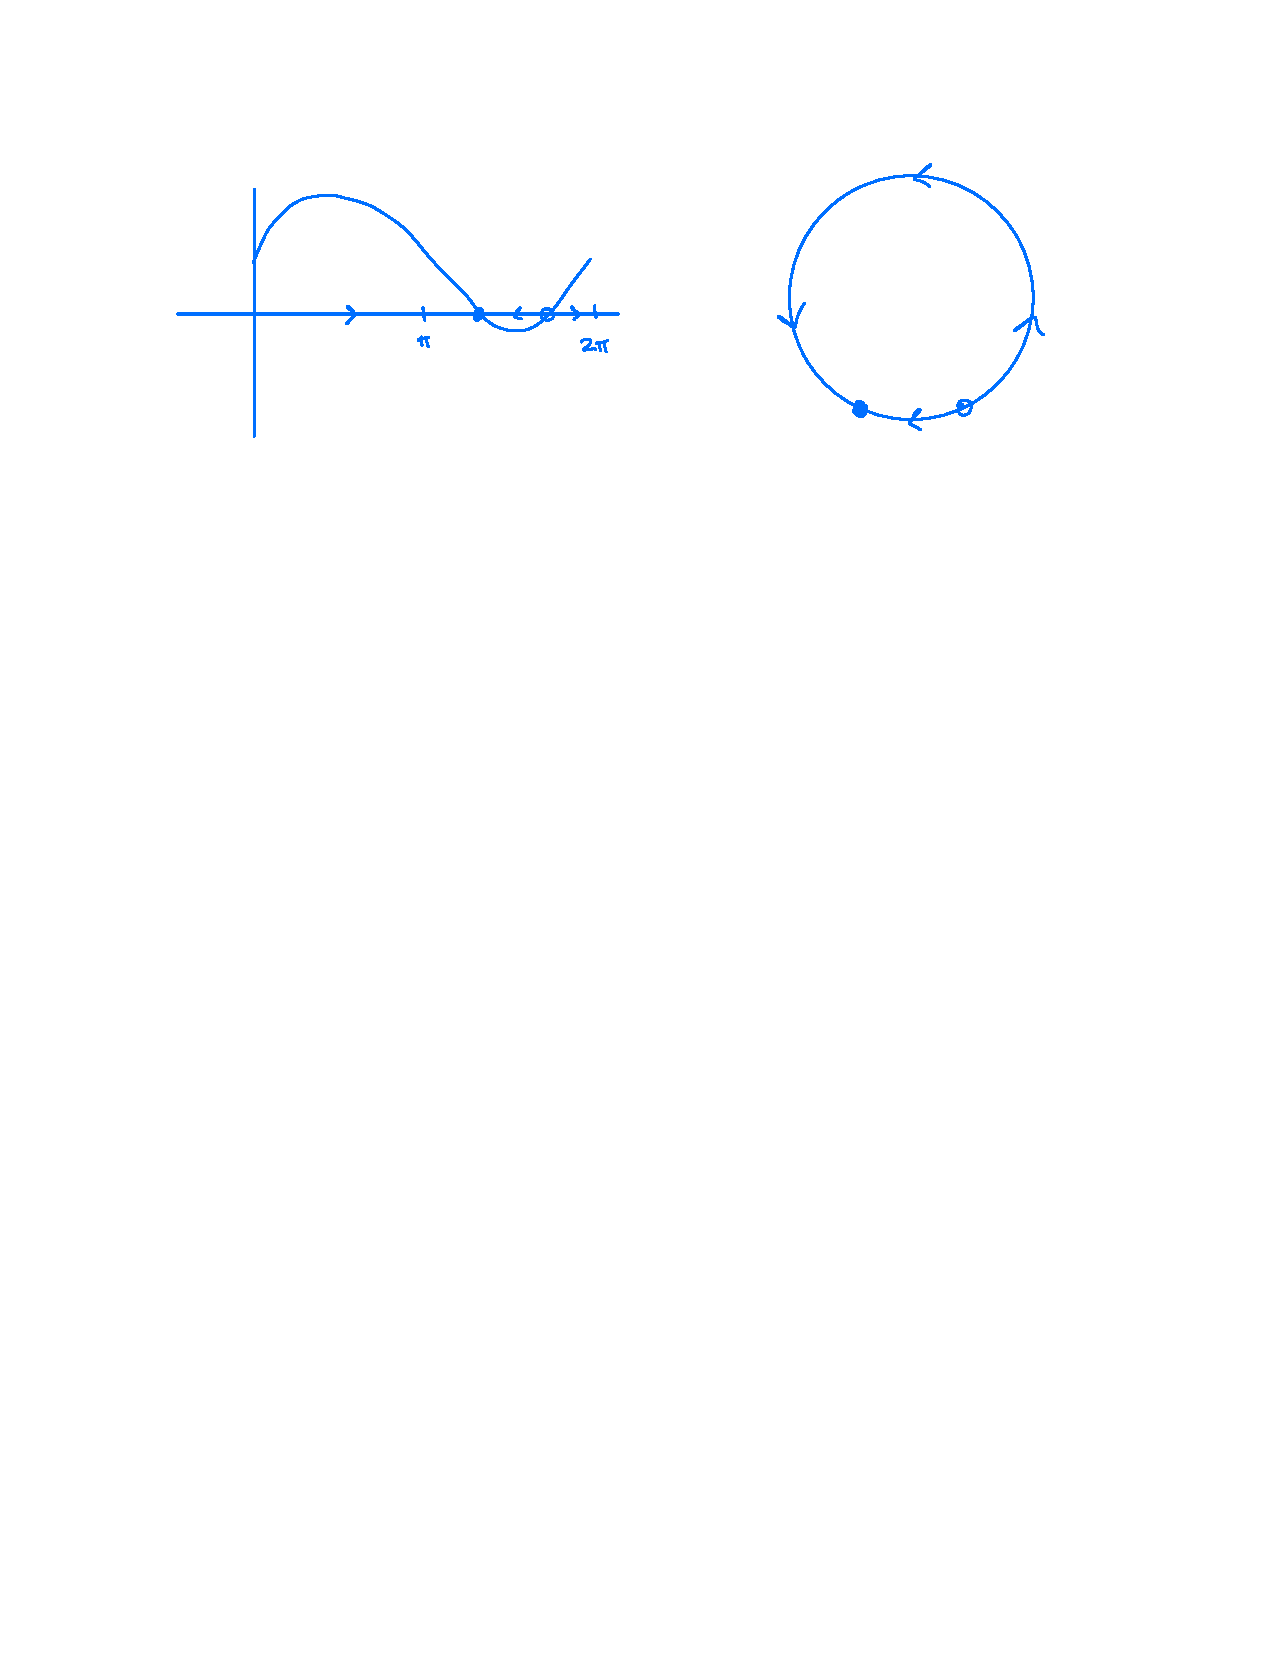
\includegraphics[width=5in]{img/H-06-2a-1}\\
The rest state is the stable equilibrium and the threshold is the unstable equilibrium. If we want to find the actual value of the stable and unstable equilibrium we would have to solve $\sin(\theta)=-\mu.$\\

Let $\delta$ denote the distance between the rest state and the threshold. If the initial condition is within $\delta$ of the rest state, then the system quickly converges to the rest state. If the initial condition is greater than $\delta$ and is on the opposite side of the threshold from the initial condition, the solution must go around the whole circle before converging to the rest state.\\
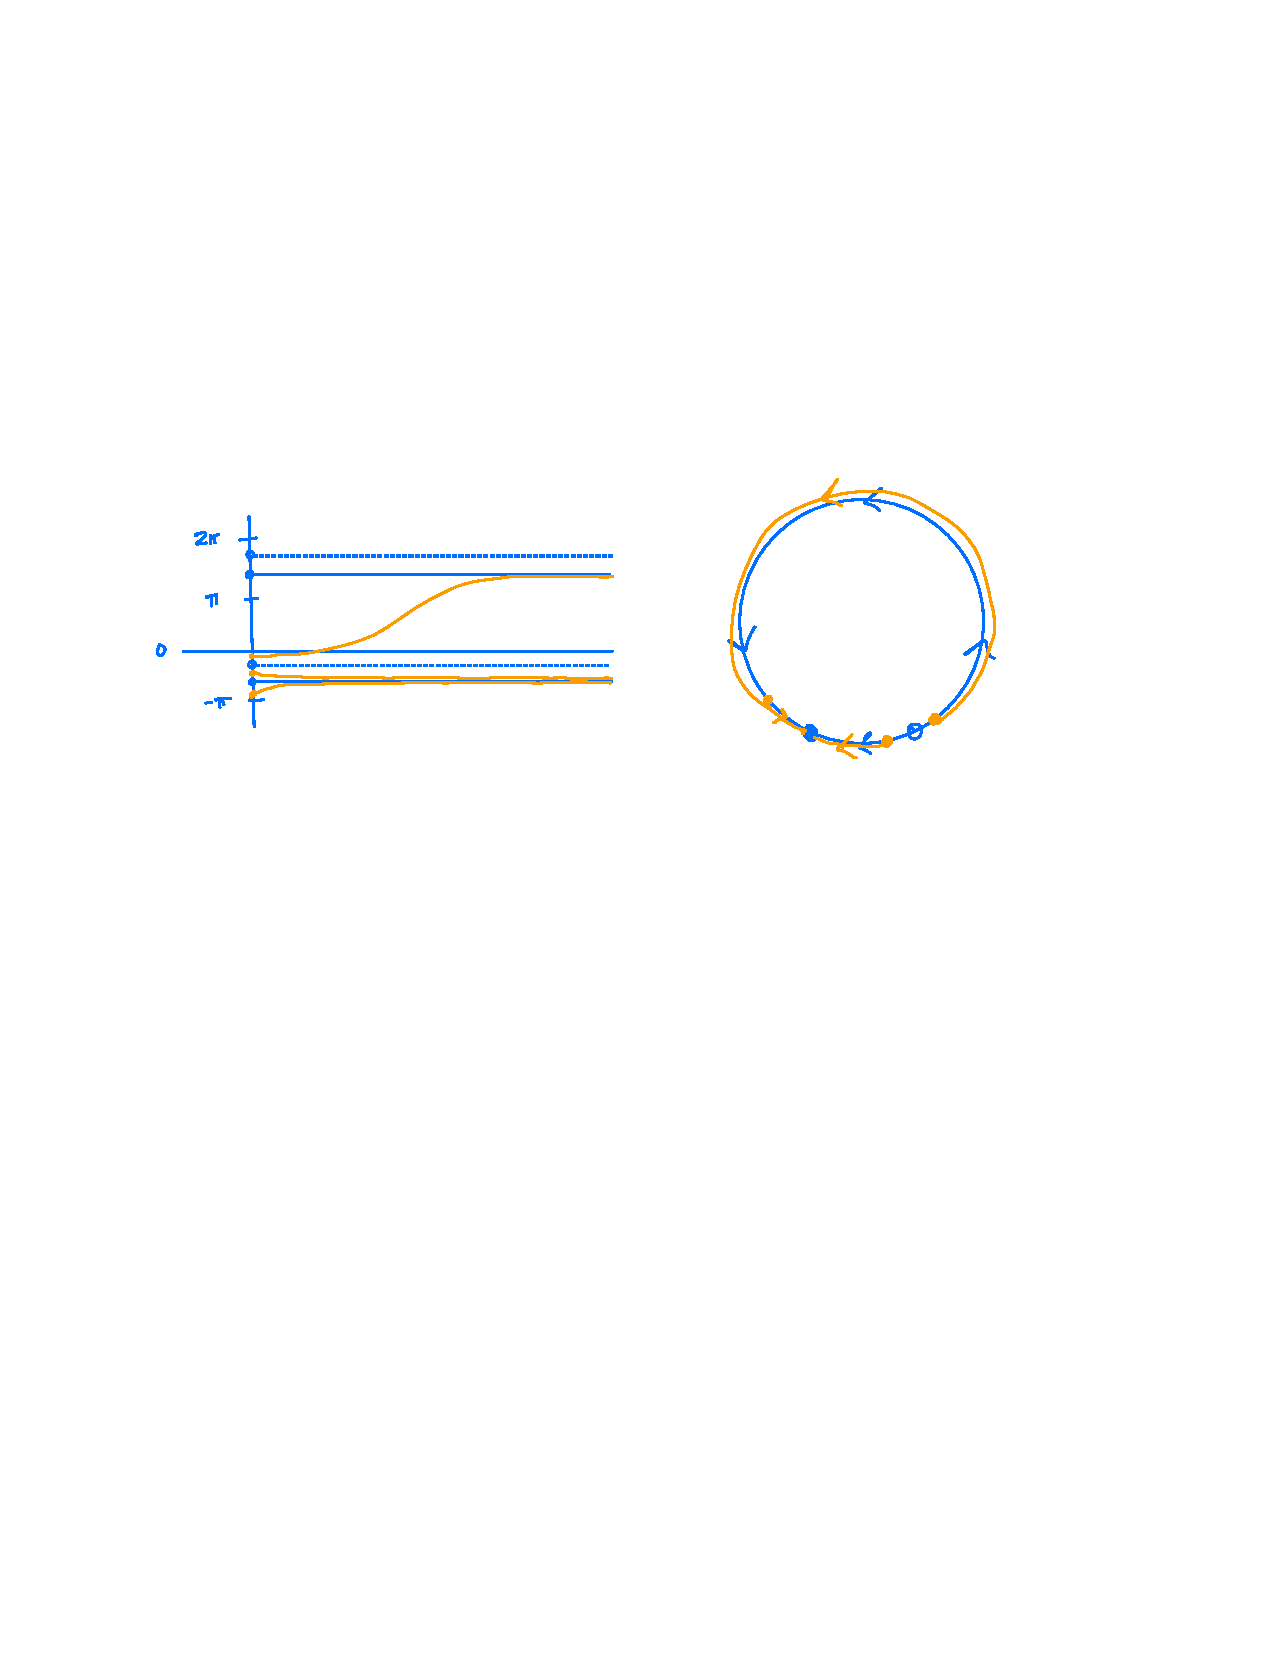
\includegraphics[width=5in]{img/H-06-2a-2}

\end{solution}


\part Do part (b) in the text as written.

\emph{In polar coordinates $x = r\cos\theta$, so $\cos\theta$ corresponds to the $x$-coordinate of motion on a unit-circle.}

\begin{solution}

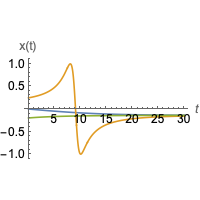
\includegraphics{img/PS06excite.png}

For initial conditions that pass the threshold, the ``voltage'' looks like a neuron (or heart) has fired and then recovered (meaning that there is a single spike).

See mathematica code.
\end{solution}
\end{parts}


% \question (7.2.12) Show that $\left\{\begin{array}{c} \dot{x} = -x + 2y^3-2y^4 \\ \dot{y} = -x-y+xy\end{array}\right.$ has no periodic solutions.  To do this, find a function $V(x,y)$ such that $\dfrac{dV}{dt}<0$ on trajectories (that are not fixed points).

% \emph{Such a function is called a Liapunov (Lyapunov) function for the system.}

% \begin{parts}
%  \item Assume you have a trajectory that is a closed orbit.  How does having $V(x,y)$ decreasing on non-fixed point trajectories lead to a contradiction?

%  \emph{Motion on a closed trajectory is periodic, so $(x(t),y(t))$ is periodic on such a trajectory.}

%     \item For the system above, try $V(x,y) = x^m + a y^n$, and choose $a, m, n$ so that it $V$ is decreasing on trajectories (i.e. so that $\frac{dV}{dt} < 0$ away from fixed points).  
    
%     \emph{Note: $m$ and $n$ will be even numbers.}

%     \emph{You are welcome to use Mathematica/Python to aid in this; be sure to describe your setup in your writeup and to submit your code.}
   
% \end{parts}









% \question (7.2.18) Consider the predator-prey model 
% \begin{align*}
% \dot{x} = & r x (1-x/2) -\frac{2x}{1+x}y \\
% \dot{y} = & -y + \frac{2x}{1+x} y \\
% & r>0 \quad x,y\geq 0
% \end{align*}
% \begin{parts}
% \item What is the long term behavior of each population in the absence of the other?  Which species is the predator and which is the prey?  How do you know?
% \item Working analytically or in Mathematica, find the fixed points of the system. Use Mathematica to classify these fixed points as stable/unstable/saddle points based on their trace and determinant.  Include the trace / determinant info in your writeup.  In addition, plot the points on axes that have appropriate labels and unit markings.

% \emph{Some code to help with plotting, or you can work by hand:} 
% \begin{verbatim}
% f[x_,y_] = {r x (1-x/2) -(2x y)/(1+x), -y + (2x y)/(1+x)}
% soln = Solve[f[x, y] == 0, {x, y}]
% r0 = 5;
% ListPlot[{x, y} /. soln /. r -> r0, 
%  Ticks -> {Automatic, {{0, 0}, {r0/4, r/4}, {r0/2, r/2}, {3 r0/4, 
%      3 r/4}, {r0, r}}}, PlotStyle -> PointSize[Large]]
% \end{verbatim} 
% \item Explain the fixed points in the context of the problem.  What does each fixed point represent in the context of the problem and what seems to be the long term behavior of the system?
% \item According to index theory, what constraints are there on limit cycles in this system?
% \item Try to use the Bendixson criterion to show that there are not limit cycles in the system.  Find the curve(s) on which $\displaystyle\nabla\cdot \left(\begin{array}{c} \dot{x} \\ \dot{y}\end{array}\right) = 0$, write it/them in the form $y = h(x)$.  Explain why this criterion does not rule out limit cycles.
% \item Now try rescaling the vector field to see if we can use Dulac's criterion to rule out limit cycles.  Rescale the vectors in the vector field using a function of the form $\displaystyle g(x,y) = \frac{1+x}{x}y^{\alpha-1}$.  Make a suitable choice of $\alpha$ so that you can use Dulac's criterion to rule out limit cycles.

% \end{parts}

\end{questions}

\vfill

\noindent\textbf{Project timeline} (See PSet 05 for topic info)

\noindent\textbf{March 22} (Wednesday) project topic + team preferences submitted during class

\noindent\textbf{March 24} (Friday) teams assigned (usually teams of 3)

\noindent\textbf{March 31} (Friday) project proposal

\noindent\textbf{Weekly on Fridays in April} Individual project work log due: this is the core individual deliverable of the project work.

\noindent\textbf{April 19} (Wednesday) team progress report slides due

\noindent\textbf{April 21/24/26} (Friday/Monday/Wednesday) team progress report presentations

\noindent\textbf{May 10, 9am} (Wednesday) team final presentation slides due

\noindent\textbf{May 10, 2pm-5pm} (Wednesday) team final presentations; final individual log due



\end{document}
